\section{Módulo de Integração}

O Módulo de Integração é responsável pela integração do Sistema TRUE  com o Middleware \textit{UbiquitOS}. Tal integração foi dificultada pelo fato do middleware ter sido desenvolvido em JAVA e o Sistema TRUE em C++. Então, para integra-los foi desenvolvido um driver no middleware que se comunica com o sistema. Tal driver foi nomeado de \textit{UserDriver} cujo diagrama de classe é mostrado na Figura~\ref{fig:userdriver}.

	\begin{figure}[hbt]
		\begin{center}
			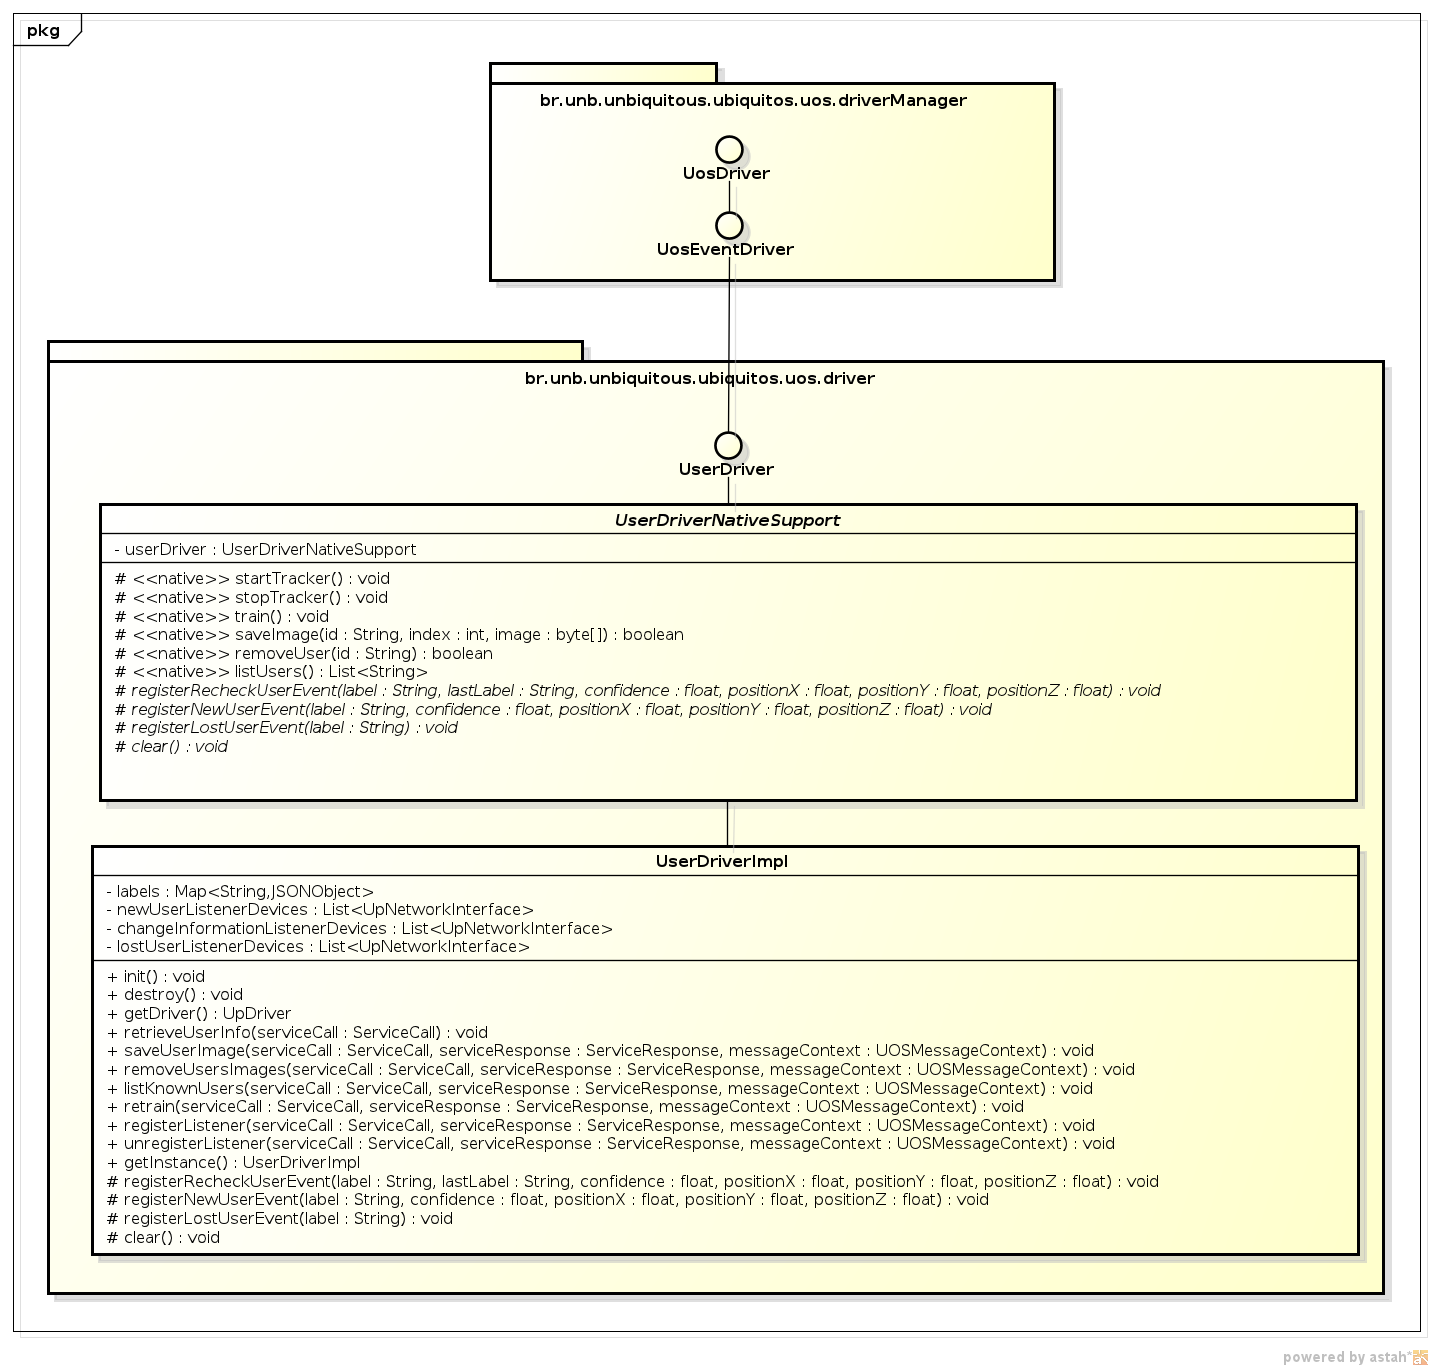
\includegraphics[scale=0.45]{figuras/4.ProblemaEProposta/diagrama-classe-userdriver.png}
		\end{center}
		\caption{Diagrama de Classe do UserDriver.}
		\label{fig:userdriver}
	\end{figure}

Os métodos do \textit{UserDriver} podem ser divididos basicamente em três grupos: métodos de inicialização, métodos nativos e serviços:

\begin{itemize}
	\item \textbf{Métodos de Inicialização}: métodos responsáveis pela inicialização do Sistema TRUE e pelo registro dos serviços que o driver possui e os eventos que pode gerar.

	\item \textbf{Métodos Nativos}: métodos declarados no driver que permitem acessar alguns métodos implementados pelo Sistema TRUE. Tais métodos permitem que o \textit{UserDriver} tenha controle sobre o sistema, podendo inicia-lo, encerra-lo, retreina-lo e, até mesmo, cadastrar e remover novos usuários a qualquer momento. Para poder implementar os métodos nativos foi utilizado JNI (\textit{Java Native Interface}), descrito no Apêndice~\ref{apend:jni}.

	\item \textbf{Serviços}: são os métodos que implementam os serviços que o \textit{UserDriver} disponibiliza as aplicações presentes no ambiente. Nestes serviços incluem consultas as informações (nome e localização) de qualquer usuário presente no ambiente, listagem dos usuários no ambiente, cadastro e remoção de novos usuário do Sistema TRUE e retreino do mesmo, e registro de \textit{listeners} que ``escutam'' os eventos gerados pelo driver.
\end{itemize}

O Módulo de Integração comunica diretamente com os Módulos de Rastreamento e de Registro através do \textit{UserDriver}. A comunicação com o Módulo de Registro acontece somente quando alguma aplicação deseja cadastrar ou remover usuários. Já a comunicação com o Módulo de Rastreamento acontece quase a todo momento: 

	\begin{itemize}
		\item a cada 5 segundos o Módulo de Rastreamento envia informações correntes sobre todos os usuários no ambiente atualizando as informações que o Módulo de Integração detém;
		\item sempre que um usuário entra ou sai do ambiente o Módulo de Rastreamento informa o Módulo de Integração;
	\end{itemize} 

Através do \textit{UserDriver}, o Middleware \textit{UbiquitOS} consegue ter acesso as informações sobre identidade e localização dos usuários presentes no ambiente em tempo real. Tais informações ficam disponíveis a qualquer aplicação registrada no middleware. 
